\begin{adjustwidth*}{}{-2.25in}
\textbf{{\large Exercises}}
\setlength{\columnsep}{25pt}
\begin{multicols*}{2}
\noindent Terms and Concepts \small
\begin{enumerate}[1)]
\item What is ``total signed area''?
\item What is ``displacement''?
\item What is $\ds \int_3^3 \sin (x)\ dx$?
\item Give a single definite integral that has the same value as 

$\ds \int_0^1(2x+3)\ dx + \int_1^2 (2x+3)\ dx$.
\end{enumerate} 

\noindent {\normalsize Problems} \small

\noindent{\bf In exercises 5--9, a graph of a function $f(x)$ is given.  Using the geometry of the graph, evaluate the definite integral.}

\begin{enumerate}[1),resume]
\item \noindent
\begin{minipage}{\linewidth}
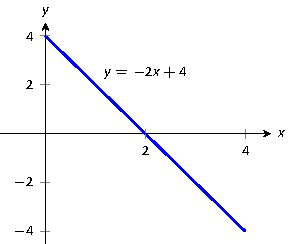
\includegraphics[scale=.8]{figures/fig05_02_ex_05}
\end{minipage}
\bmtwo
\begin{enumerate}
\item		$\ds \int_0^1 (-2x+4)\ dx$
\item		$\ds \int_0^2 (-2x+4)\ dx$
\item		$\ds \int_0^3 (-2x+4)\ dx$
\item		$\ds \int_1^3 (-2x+4)\ dx$
\item		$\ds \int_2^4 (-2x+4)\ dx$
\item		$\ds \int_0^1 (-6x+12)\ dx$
\end{enumerate}
\emtwo

\item\noindent
\begin{minipage}{\linewidth}
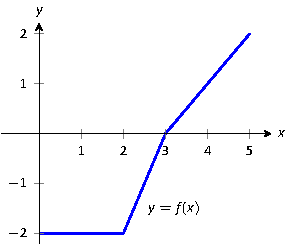
\includegraphics[scale=.8]{figures/fig05_02_ex_06}
\end{minipage}
\bmtwo
\begin{enumerate}
\item		$\ds \int_0^2 f(x)\ dx$
\item		$\ds \int_0^3 f(x)\ dx$
\item		$\ds \int_0^5 f(x)\ dx$
\item		$\ds \int_2^5 f(x)\ dx$
\item		$\ds \int_5^3 f(x)\ dx$
\item		$\ds \int_0^3 -2f(x)\ dx$
\end{enumerate}
\emtwo

\item \noindent
\begin{minipage}{\linewidth}
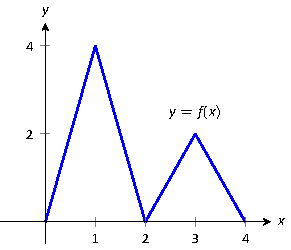
\includegraphics[scale=.8]{figures/fig05_02_ex_07}
\end{minipage}
\bmtwo
\begin{enumerate}
\item		$\ds \int_0^2 f(x)\ dx$
\item		$\ds \int_2^4 f(x)\ dx$
\item		$\ds \int_2^4 2f(x)\ dx$
\item		$\ds \int_0^1 4x\ dx$
\item		$\ds \int_2^3 (2x-4)\ dx$
\item		$\ds \int_2^3 (4x-8)\ dx$
\end{enumerate}
\emtwo

\item \noindent
\begin{minipage}{\linewidth}
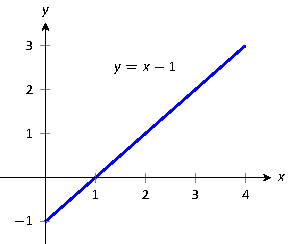
\includegraphics[scale=.8]{figures/fig05_02_ex_08}
\end{minipage}
\bmtwo
\begin{enumerate}
\item		$\ds \int_0^1 (x-1)\ dx$
\item		$\ds \int_0^2 (x-1)\ dx$
\item		$\ds \int_0^3 (x-1)\ dx$
\item		$\ds \int_2^3 (x-1)\ dx$
\item		$\ds \int_1^4 (x-1)\ dx$
\item		$\ds \int_1^4 \big((x-1)+1\big)\ dx$
\end{enumerate}
\emtwo

\item \noindent
\begin{minipage}{\linewidth}
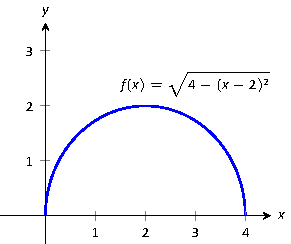
\includegraphics[scale=.8]{figures/fig05_02_ex_09}
\end{minipage}
\bmtwo
\begin{enumerate}
\item		$\ds \int_0^2 f(x)\ dx$
\item		$\ds \int_2^4 f(x)\ dx$
\item		$\ds \int_0^4 f(x)\ dx$
\item		$\ds \int_0^4 5f(x)\ dx$
\end{enumerate}
\emtwo
\end{enumerate}

\noindent{\bf In exercises 10--13, a graph of a function $f(x)$ is given; the numbers inside the shaded regions give the area of that region.  Evaluate the definite integrals using this area information.}

\begin{enumerate}[1),resume]
\item \noindent
\begin{minipage}{\linewidth}
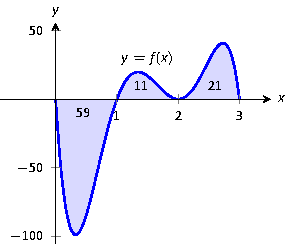
\includegraphics[scale=.8]{figures/fig05_02_ex_10}
\end{minipage}
\bmtwo
\begin{enumerate}
\item		$\ds \int_0^1 f(x)\ dx$
\item		$\ds \int_0^2 f(x)\ dx$
\item		$\ds \int_0^3 f(x)\ dx$
\item		$\ds \int_1^2 -3f(x)\ dx$
\end{enumerate}
\emtwo


\end{enumerate}

%------------------------------------------
% END OF EXERCISES ON FIRST PAGE
%------------------------------------------
\end{multicols*}
\end{adjustwidth*}

\clearpage

\begin{adjustwidth*}{}{-2.25in}
\setlength{\columnsep}{25pt}
\begin{multicols*}{2}\small

\begin{enumerate}[1),start=11]
\item \noindent
\begin{minipage}{\linewidth}
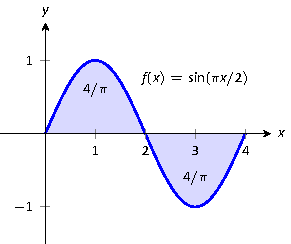
\includegraphics[scale=.8]{figures/fig05_02_ex_11}
\end{minipage}
\bmtwo
\begin{enumerate}
\item		$\ds \int_0^2 f(x)\ dx$
\item		$\ds \int_2^4 f(x)\ dx$
\item		$\ds \int_0^4 f(x)\ dx$
\item		$\ds \int_0^1 f(x)\ dx$
\end{enumerate}
\emtwo

\item \noindent
\begin{minipage}{\linewidth}
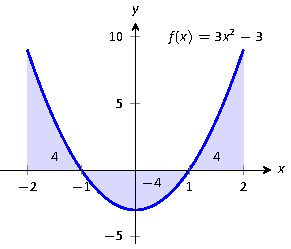
\includegraphics[scale=.8]{figures/fig05_02_ex_12}
\end{minipage}
\bmtwo
\begin{enumerate}
\item		$\ds \int_{-2}^{-1} f(x)\ dx$
\item		$\ds \int_1^2 f(x)\ dx$
\item		$\ds \int_{-1}^1 f(x)\ dx$
\item		$\ds \int_0^1 f(x)\ dx$
\end{enumerate}
\emtwo

\item \noindent
\begin{minipage}{\linewidth}
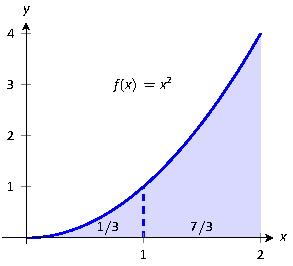
\includegraphics[scale=.8]{figures/fig05_02_ex_13}
\end{minipage}
\bmtwo
\begin{enumerate}
\item		$\ds \int_{0}^{2} 5x^2\ dx$
\item		$\ds \int_0^2 (x^2+3)\ dx$
\item		$\ds \int_{1}^3 (x-1)^2\ dx$
\item		$\ds \int_2^4 \big((x-2)^2+5\big)\ dx$
\end{enumerate}
\emtwo

\end{enumerate}

\noindent{\bf In exercises 14--17, let
\bmtwo
\begin{itemize}
\item $\ds \int_0^2 f(x) \ dx = 5,$
\item $\ds \int_0^3 f(x) \ dx = 7,$
\item $\ds \int_0^2 g(x) \ dx = -3$, and
\item $\ds \int_2^3 g(x) \ dx = 5.$
\end{itemize}
\emtwo
Use these values to evaluate the given definite integrals.}

\begin{enumerate}[1),resume]
\item $\ds \int_0^2 \big(f(x)+g(x)\big) \ dx$
\item $\ds \int_0^3 \big(f(x)-g(x)\big) \ dx$
\item $\ds \int_2^3 \big(3f(x)+2g(x)\big) \ dx$
\item Find values for $a$ and $b$ such that 

$\ds \int_0^3 \big(af(x)+bg(x)\big) \ dx=0$
\end{enumerate}

\noindent{\bf In exercises 18--21, let 
\bmtwo
\begin{itemize}
\item $\ds \int_0^3 s(t) \ dt = 10,$
\item $\ds \int_3^5 s(t) \ dx = 8,$
\item $\ds \int_3^5 r(t) \ dx = -1$, and
\item $\ds \int_0^5 r(t) \ dx = 11.$
\end{itemize}
\emtwo
Use these values to evaluate the given definite integrals.}

\begin{enumerate}[1),resume]
\item $\ds \int_0^3 \big(s(t) + r(t)\big)\ dt$
\item $\ds \int_5^0 \big(s(t) - r(t)\big)\ dt$
\item $\ds \int_3^3 \big(\pi s(t) - 7r(t)\big)\ dt$
\item Find values for $a$ and $b$ such that 

$\ds \int_0^5 \big(ar(t)+bs(t)\big) \ dt=0$

 \item The velocity of an object moving along an axis is given by the piecewise linear function $v$ that is pictured below.  Assume that the object is moving to the right when its velocity is positive, and moving to the left when its velocity is negative.  Assume that the given velocity function is valid for $t = 0$ to $t = 4$.
\begin{center}
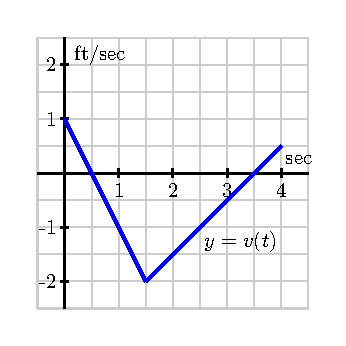
\includegraphics[scale=.75]{figures/4_3_Ez1.eps}
\end{center}
	\ba
		\item Write an expression involving definite integrals whose value is the total change in position of the object on the interval $[0,4]$.
		\item Use the provided graph of $v$ to determine the value of the total change in position on $[0,4]$.
		\item Write an expression involving definite integrals whose value is the total distance traveled by the object on $[0,4]$.  What is the exact value of the total distance traveled on $[0,4]$?
		\item What is the object's exact average velocity on $[0,4]$?
		\item Find an algebraic formula for the object's position function on $[0, 1.5]$ that satisfies $s(0) = 0$.
	\ea
\end{enumerate}

%---------------------------------------------
% END OF EXERCISES ON SECOND PAGE
%---------------------------------------------
\end{multicols*}
\end{adjustwidth*}

\afterexercises